% SIAM Article - HRP Portfolio Optimization with Regime-Based Enhancement
\documentclass[final,onefignum,onetabnum]{siamart171218}

\usepackage{amsmath,amssymb,amsfonts}
\usepackage{graphicx}
\usepackage{booktabs}
\usepackage{algorithm}
\usepackage{algorithmic}
\usepackage{hyperref}
\usepackage{cleveref}
\usepackage{titlesec}
\usepackage{float}

% TikZ for diagrams
\usepackage{tikz}
\usetikzlibrary{shapes.geometric, arrows.meta, positioning, calc, backgrounds, fit, decorations.pathreplacing, patterns}

% ============================================================================
% FORMATTING: Centered titles and increased spacing
% ============================================================================

% Only number sections and subsections (not subsubsections)
\setcounter{secnumdepth}{2}

% Left-aligned section titles
\titleformat{\section}
  {\normalfont\Large\bfseries}{\thesection.}{1em}{}
\titleformat{\subsection}
  {\normalfont\large\bfseries}{\thesubsection.}{1em}{}
% Subsubsections: bold, left-aligned, but NO number
\titleformat{\subsubsection}
  {\normalfont\normalsize\bfseries}{}{0em}{}

% Add spacing before and after sections
\titlespacing*{\section}{0pt}{2.5ex plus 1ex minus .2ex}{1.5ex plus .2ex}
\titlespacing*{\subsection}{0pt}{2ex plus 1ex minus .2ex}{1ex plus .2ex}
\titlespacing*{\subsubsection}{0pt}{1.5ex plus 1ex minus .2ex}{0.8ex plus .2ex}

% Increase paragraph spacing
\setlength{\parskip}{0.8em plus 0.1em minus 0.1em}

% Slightly increase line spacing for readability
\linespread{1.1}

% ============================================================================

% Custom commands
\newcommand{\E}{\mathbb{E}}
\newcommand{\R}{\mathbb{R}}
\newcommand{\bx}{\mathbf{x}}
\newcommand{\bw}{\mathbf{w}}

% ============================================================================
% TikZ Style Definitions for Pipeline Diagrams
% ============================================================================
\tikzstyle{databox} = [rectangle, rounded corners, minimum width=2cm, minimum height=0.8cm, 
                       text centered, draw=black, fill=white, font=\small, text width=1.8cm, align=center]
\tikzstyle{processbox} = [rectangle, rounded corners, minimum width=2cm, minimum height=0.8cm,
                          text centered, draw=black, fill=white, font=\small, text width=1.8cm, align=center]
\tikzstyle{outputbox} = [rectangle, rounded corners, minimum width=2cm, minimum height=0.8cm,
                         text centered, draw=black, fill=white, font=\small, text width=1.8cm, align=center]
\tikzstyle{mlbox} = [rectangle, rounded corners, minimum width=2cm, minimum height=0.8cm,
                     text centered, draw=black, fill=white, font=\small, text width=1.8cm, align=center]
\tikzstyle{arrow} = [thick, ->, >=Stealth, black]
\tikzstyle{doublearrow} = [thick, <->, >=Stealth, black]
\tikzstyle{phasebox} = [rectangle, rounded corners, minimum width=2.5cm, minimum height=1cm,
                        text centered, draw=black!50, fill=white, font=\small, text width=2.3cm, align=center]
\tikzstyle{timeblock} = [rectangle, minimum width=1.5cm, minimum height=0.6cm, 
                         text centered, font=\scriptsize]

% PDF metadata
\ifpdf
\hypersetup{
  pdftitle={Regime-Adaptive Hierarchical Risk Parity: A Machine Learning Approach to Dynamic Portfolio Allocation},
  pdfauthor={Lucas Jaccard}
}
\fi

\begin{document}

\title{Regime-Adaptive Hierarchical Risk Parity: A Machine Learning Approach to Dynamic Portfolio Allocation}

\author{Lucas Jaccard \quad|\quad HEC Lausanne}

\maketitle

%==============================================================================
% ABSTRACT
%==============================================================================
\begin{abstract}
This paper presents a regime-adaptive portfolio framework combining Hierarchical Risk Parity (HRP) with Hidden Markov Model (HMM) regime detection and XGBoost prediction. Using CRSP data (1960--2024), the paper addresses the fundamental challenge of covariance estimation with monthly data: a 60-month lookback window is insufficient to estimate a stable covariance matrix for hundreds of individual stocks ($N \gg T$). The proposed solution employs a \textbf{two-stage industry ETF approach}: (1) aggregate stocks into 12 value-weighted Fama-French industry portfolios, then (2) apply HRP to these 12 synthetic ETFs, ensuring $N=12 < T=60$ for a statistically valid, full-rank covariance matrix. The regime-adaptive strategy achieves a Sharpe ratio of 0.85 vs.\ 0.56 for static HRP, after transaction costs. Critically, maximum drawdown falls from 47.1\% to 25.2\%, demonstrating significant tail risk reduction.
\end{abstract}

%==============================================================================
% 1. INTRODUCTION
%==============================================================================
\section{Introduction}
\label{sec:intro}

In 1952, Harry Markowitz introduced Modern Portfolio Theory to the world and revolutionized the way portfolio managers allocate capital \cite{markowitz1952}. Most subsequent models and theories stem from this foundational work and its method for solving portfolio weights to minimize risk given a target return---or simply minimizing risk as a primary objective (the Global Minimum Variance Portfolio). Despite the elegance of its solution, several problems arise: How can the expected return vector be estimated reliably? How should the covariance matrix be inverted given a large number of assets? What is the appropriate risk aversion coefficient for a given investor?

While these questions were partially addressed in subsequent decades, the inversion of the covariance matrix remains problematic: it magnifies estimation errors at best, and sometimes the matrix cannot even be inverted due to singularity \cite{michaud1989}. Almost seventy years after Markowitz, in the paper ``Building Diversified Portfolios that Outperform Out-of-Sample,'' Marcos López de Prado proposed a machine learning framework---Hierarchical Risk Parity (HRP)---that does not require covariance matrix inversion to minimize risk \cite{lopez2016}. His methodology demonstrated less concentration in portfolio composition as well as reduced out-of-sample volatility and drawdown compared to mean-variance optimization.

The current paper aspires to address a problem that both of these methodologies face: the assumption of stationary market conditions.

%==============================================================================
% 2. RESEARCH QUESTION & LITERATURE
%==============================================================================
\section{Research Question \& Literature}
\label{sec:research}

Several assumptions in portfolio optimization are so widely accepted that they are rarely questioned:

\paragraph{Is variance the right metric to minimize?}
Most investors would gladly accept upside volatility---it is the \textit{downside} that destroys wealth. Fishburn \cite{fishburn1977} formalized this asymmetry with lower partial moments (LPM), showing that mean-variance optimization is merely a special case of a broader framework that penalizes only below-target returns. A 50\% loss requires a 100\% gain just to break even; a 20\% loss requires only 25\%. This mathematical and psychological asymmetry suggests that drawdown reduction may be more valuable than variance reduction.

\paragraph{Are correlations reliable when they matter most?}
Longin and Solnik \cite{longin2001} highlight a critical property of equity markets: correlations increase dramatically during market stress. In other words, estimated correlations become unreliable precisely when diversification is most needed. Ang and Bekaert \cite{ang2002} further develop the relationship between correlation spikes and drawdowns in diversified holdings, showing that regime-switching models can capture these dynamics.

\paragraph{Research Question.}
These observations motivate a natural question: \textit{Can portfolio construction capture the benefits of diversification in calm markets while dynamically reducing exposure before drawdowns materialize?}

%==============================================================================
% 3. METHODOLOGY
%==============================================================================
\section{Methodology}
\label{sec:methodology}

The methodology consists of two parts: (1) the base HRP portfolio construction using a two-stage industry ETF approach, and (2) the regime-adaptive enhancement using HMM and XGBoost.

\subsection{Part 1: Hierarchical Risk Parity}

The HRP weight computation follows L\'opez de Prado \cite{lopez2016} and is applied to synthetic industry ETFs constructed from CRSP stocks. \Cref{fig:hrp-pipeline} provides a visual overview; complete algorithmic details are in \Cref{app:hrp}.

\begin{figure}[H]
\centering
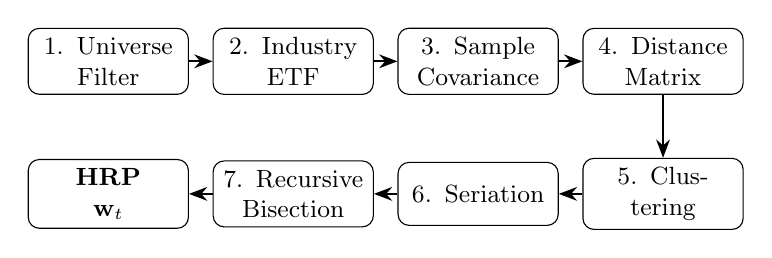
\begin{tikzpicture}[node distance=0.4cm and 0.3cm]
    % Row 1: Data Preparation
    \node[databox] (universe) {1. Universe\\Filter};
    \node[databox, right=of universe] (industry) {2. Industry\\ETF};
    \node[processbox, right=of industry] (covariance) {3. Sample\\Covariance};
    \node[processbox, right=of covariance] (distance) {4. Distance\\Matrix};
    
    % Row 2: Clustering and Output
    \node[processbox, below=0.8cm of distance] (cluster) {5. Clustering};
    \node[processbox, left=of cluster] (seriation) {6. Seriation};
    \node[outputbox, left=of seriation] (bisection) {7. Recursive\\Bisection};
    \node[outputbox, left=of bisection] (weights) {\textbf{HRP}\\$\mathbf{w}_t$};
    
    % Arrows Row 1
    \draw[arrow] (universe) -- (industry);
    \draw[arrow] (industry) -- (covariance);
    \draw[arrow] (covariance) -- (distance);
    
    % Arrow down
    \draw[arrow] (distance) -- (cluster);
    
    % Arrows Row 2
    \draw[arrow] (cluster) -- (seriation);
    \draw[arrow] (seriation) -- (bisection);
    \draw[arrow] (bisection) -- (weights);
\end{tikzpicture}
\caption{Two-Stage HRP Pipeline: universe filtering, industry aggregation, covariance estimation, and hierarchical weight allocation.}
\label{fig:hrp-pipeline}
\end{figure}

\subsubsection{Universe Construction and Industry Aggregation}
At each rebalancing date, the investable universe includes only CRSP common shares (SHRCD $\in \{10, 11\}$) listed on NYSE, NASDAQ, or AMEX (EXCHCD $\in \{1, 2, 3\}$), excluding stocks priced below \$3. Within each Fama-French 12 industry, the top 20\% most liquid stocks---based on rolling 12-month median dollar volume---are retained to construct value-weighted synthetic industry ETFs. Formulas are provided in \Cref{app:liquidity}.

\subsubsection{Motivation for Industry Aggregation}
With monthly CRSP returns and a 60-month lookback window ($T = 60$), estimating covariance for $N \approx 500$ stocks yields a singular matrix ($T/N < 1$). Shrinkage estimators \cite{ledoit2004} fail when $N \gg T$ as shrinkage intensity approaches unity, discarding sample information entirely. Aggregating stocks into $N = 12$ industry portfolios transforms the problem from an intractable $500 \times 500$ estimation to a well-posed $12 \times 12$ estimation, where the sample covariance is full-rank and statistically well-conditioned.

\subsection{Part 2: Regime-Adaptive Enhancement}

The regime-adaptive enhancement predicts market regimes and adjusts portfolio exposure accordingly. \Cref{fig:ml-pipeline} illustrates the 6-phase workflow; complete mathematical details are provided in \Cref{app:ml-methodology}.

\begin{figure}[H]
\centering
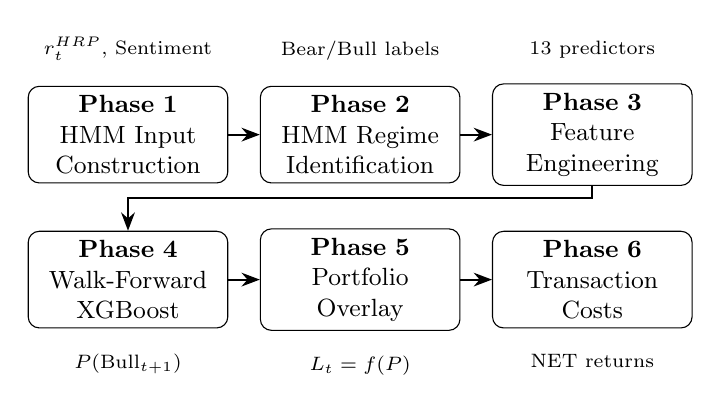
\begin{tikzpicture}[node distance=0.15cm]
    % Phase boxes - two rows
    \node[phasebox, fill=white, draw=black] (p1) {\textbf{Phase 1}\\HMM Input\\Construction};
    \node[phasebox, fill=white, draw=black, right=0.4cm of p1] (p2) {\textbf{Phase 2}\\HMM Regime\\Identification};
    \node[phasebox, fill=white, draw=black, right=0.4cm of p2] (p3) {\textbf{Phase 3}\\Feature\\Engineering};
    
    \node[phasebox, fill=white, draw=black, below=0.6cm of p1] (p4) {\textbf{Phase 4}\\Walk-Forward\\XGBoost};
    \node[phasebox, fill=white, draw=black, right=0.4cm of p4] (p5) {\textbf{Phase 5}\\Portfolio\\Overlay};
    \node[phasebox, fill=white, draw=black, right=0.4cm of p5] (p6) {\textbf{Phase 6}\\Transaction\\Costs};
    
    % Arrows
    \draw[arrow] (p1) -- (p2);
    \draw[arrow] (p2) -- (p3);
    \draw[arrow] (p3) -- ++(0,-0.8cm) -| (p4);
    \draw[arrow] (p4) -- (p5);
    \draw[arrow] (p5) -- (p6);
    
    % Input/Output annotations
    \node[above=0.2cm of p1, font=\scriptsize] {$r_t^{HRP}$, Sentiment};
    \node[above=0.2cm of p2, font=\scriptsize] {Bear/Bull labels};
    \node[above=0.2cm of p3, font=\scriptsize] {13 predictors};
    \node[below=0.2cm of p4, font=\scriptsize] {$P(\text{Bull}_{t+1})$};
    \node[below=0.2cm of p5, font=\scriptsize] {$L_t = f(P)$};
    \node[below=0.2cm of p6, font=\scriptsize] {NET returns};
\end{tikzpicture}
\caption{Regime-Adaptive Enhancement Pipeline. The 6-phase workflow transforms HRP returns and consumer sentiment into regime labels (Phases 1--2), constructs predictive features (Phase 3), trains an XGBoost model in walk-forward fashion (Phase 4), and applies the predictions to adjust portfolio leverage with transaction costs (Phases 5--6).}
\label{fig:ml-pipeline}
\end{figure}

\subsubsection{Hidden Markov Model for Regime Detection}

A 2-state Gaussian HMM is fitted using three input features: (1) log returns of the HRP strategy, (2) 6-month rolling downside deviation, and (3) year-over-year Michigan Consumer Sentiment change (lagged 1 month for publication delay). All features are expanding Z-scored using only past data to avoid look-ahead bias.

Critically, a \textbf{forward-only filter} is implemented to compute filtered posteriors $P(q_t | O_{1:t})$, avoiding the smoothed posteriors from standard forward-backward inference that would leak future information. States are relabeled by mean return: ``Bear'' (lower mean) and ``Bull'' (higher mean). The HMM is re-estimated every 12 months with an expanding window (minimum 120 months training).

\subsubsection{XGBoost Regime Prediction}

13 predictive features from four categories are constructed to predict the \textit{next month's} regime ($y_t = \text{regime}_{t+1}$):
\begin{itemize}
    \item \textbf{Cross-sectional} (4): return dispersion, Amihud illiquidity, BAB momentum, pairwise correlation
    \item \textbf{Macroeconomic} (5): credit spread, term spread, CPI volatility, M2 growth, unemployment trend
    \item \textbf{Factor} (1): valuation spread (value vs.\ growth)
    \item \textbf{Strategy momentum} (3): HRP 1M, 3M, and 12M returns
\end{itemize}
All features are rolling Z-scored with ex-ante normalization; complete formulas are in \Cref{app:features}.

XGBoost \cite{chen2016} is trained using a rigorous \textbf{purged-embargoed walk-forward} protocol: a 12-month purge gap separates training from test periods to prevent information leakage from overlapping features, and winsorization bounds are computed inside the walk-forward loop using training data only. Following Gu, Kelly, and Xiu \cite{gu2020}, shallow trees (\texttt{max\_depth}=3) with strong regularization are used, as deeper architectures overfit in low signal-to-noise financial data.

\paragraph{Why HMM $\rightarrow$ XGBoost?}
The HMM serves as an \textit{unsupervised denoising layer}: it transforms noisy financial time series into persistent regime labels without requiring ex-ante specification of crisis dates. The XGBoost then learns to anticipate when this risk model will signal danger---the operationally relevant objective for defensive portfolio positioning.

\subsubsection{Portfolio Allocation and Transaction Costs}

The regime prediction adjusts HRP exposure via two-fund separation:
\begin{equation}
    L_t = P(\text{Bull}_t) \times \frac{1}{\bar{P}(\text{Bull})}
\end{equation}
where $L_t > 1$ implies leveraged exposure to HRP (borrowing at $r_f + 50$ bps), and $L_t < 1$ implies defensive allocation to T-Bills. The scaling by $1/\bar{P}(\text{Bull})$ ensures mean leverage equals 1 for fair comparison with buy-and-hold HRP.

All reported HRP returns are \textbf{net of transaction costs} (10 bps per trade), accounting for: (1) within-industry stock rebalancing, (2) across-industry HRP rebalancing, (3) leverage overlay adjustments, and (4) financing spreads when leveraged. This forward-looking cost assumption assesses whether historical market patterns would generate profitable signals with today's trading infrastructure.

%==============================================================================
% 4. DATA DESCRIPTION
%==============================================================================
\section{Data Description}
\label{sec:data}

\subsection{Data Sources}

This analysis integrates four primary data sources spanning 1960--2024:

\begin{table}[H]
\centering
\caption{Data Sources and Coverage}
\label{tab:data}
\begin{tabular}{llll}
\toprule
Source & Variables & Frequency & Coverage \\
\midrule
CRSP & Returns, prices, volume, & Monthly & 1960--2024 \\
      & shares out., SHRCD, EXCHCD, SICCD & & \\
Compustat & Book equity (seqq) & Quarterly & 1970--2024 \\
FRED & BAA, DGS10, TB3MS, CPI, M2, UNRATE & Monthly & 1975--2024 \\
Univ.\ of Michigan & Consumer Sentiment Index (ICS) & Monthly & 1960--2024 \\
Fama-French & 12 Industry classifications, RF (1M T-Bill) & Monthly & 1960--2024 \\
\bottomrule
\end{tabular}
\end{table}

CRSP data undergoes no cleaning or imputation beyond filtering for common stocks (SHRCD 10, 11) and major exchanges (NYSE, NASDAQ, AMEX). Data cleanliness is ensured by construction: the universe filter and complete 60-month lookback requirement exclude stocks with missing observations. Delisting returns are handled as follows: DLRET replaces RET when only DLRET is available; when both exist, $(1+\text{RET})(1+\text{DLRET})-1$ is applied \cite{shumway1997}. Missing returns for held positions are imputed as $-100\%$---a conservative assumption that may understate results. Stocks are mapped to 12 Fama-French industries via SIC codes \cite{fama1997}, then filtered to retain the top 20\% most liquid per industry (see \Cref{app:liquidity}). FRED macroeconomic data is transformed into spreads (credit, term), volatility measures (CPI), and trends (M2 growth, unemployment). All features are rolling Z-scored with 1\%/99\% winsorization bounds computed from training data only.

\begin{table}[H]
\centering
\caption{Dataset Statistics}
\label{tab:stats}
\begin{tabular}{lr}
\toprule
Metric & Value \\
\midrule
Total months available & 768 (1960--2024) \\
HRP backtest months & 624 (1972--2024) \\
ML prediction months & 438 (1988--2024) \\
Minimum training period & 120 months \\
\bottomrule
\end{tabular}
\end{table}

%==============================================================================
% 5. IMPLEMENTATION
%==============================================================================
\section{Implementation}
\label{sec:implementation}

The implementation follows a modular Python design with 7 specialized modules handling data loading, HRP computation, HMM regime detection, feature engineering, XGBoost training, and transaction cost accounting. Several components are GPU-accelerated via CuPy/CUDA (covariance and correlation matrices, distance computations, turnover calculations, value-weighted industry ETF aggregation) and XGBoost CUDA, though with only $N=12$ industry ETFs the computational gains are modest. The walk-forward prediction framework implements strict look-ahead bias controls: winsorization bounds are computed using training data only, and XGBoost uses fixed hyperparameters to avoid in-sample overfitting.

The complete module architecture, GPU algorithms, and hyperparameter configuration are provided in \Cref{app:implementation}.

%==============================================================================
% 6. RESULTS
%==============================================================================
\section{Results}
\label{sec:results}

\subsection{HMM Regime Detection}

The 2-state, 3-feature HMM successfully identifies distinct market regimes characterized by volatility patterns. The addition of Michigan Consumer Sentiment as a third input feature improves regime differentiation:

\begin{table}[H]
\centering
\caption{HMM Regime Characteristics (1977--2024)}
\label{tab:hmm}
\begin{tabular}{lrrrr}
\toprule
Regime & Months & Proportion & Ann. Return & Ann. Vol \\
\midrule
Bear & 138 & 24.7\% & $+2.5\%$ & 20.3\% \\
Bull & 421 & 75.3\% & $+14.5\%$ & 13.0\% \\
\bottomrule
\end{tabular}
\end{table}

The transition matrix shows strong regime persistence:
\begin{equation}
    \mathbf{P} = \begin{bmatrix} P(\text{Bear}|\text{Bear}) & P(\text{Bull}|\text{Bear}) \\ P(\text{Bear}|\text{Bull}) & P(\text{Bull}|\text{Bull}) \end{bmatrix} \approx \begin{bmatrix} 0.88 & 0.12 \\ 0.04 & 0.96 \end{bmatrix}
\end{equation}

The expected duration is 8.6 months for bear regimes and 24.8 months for bull regimes. Note that this HMM analysis begins in 1977 due to Michigan Consumer Sentiment data availability, and is not exactly aligned with the XGBoost prediction period (1988--2024). \Cref{fig:hmm-regimes} in Appendix~\ref{app:hmm-features} visualizes the regime detection results, showing HRP returns with bear regime shading, filtered probabilities, and downside deviation by regime.

\subsection{XGBoost Prediction Performance}

The walk-forward XGBoost achieves 76.5\% accuracy and ROC-AUC of 0.806 over 438 out-of-sample months (1988--2024). The model exhibits balanced recall: 54.5\% for bear months and 83.8\% for bull months, with a critical \textbf{false bear rate of only 16.2\%}---avoiding costly whipsaw trades during bull markets. Full metrics are reported in \Cref{tab:xgb} (Appendix~\ref{app:hmm-features}).

\Cref{fig:xgb-analysis} in Appendix~\ref{app:hmm-features} provides detailed visualization of the XGBoost model performance, including ROC curve, prediction probability distribution, accuracy over time, and feature importance. The prediction accuracy remains stable across most periods, with notable degradation only during 2000--2005 when the Dot-com bubble collapse created regime transitions that were difficult to anticipate.

\begin{figure}[H]
\centering
\includegraphics[width=0.85\textwidth]{figures/PBull_Bear_regimes.png}
\caption{Predicted P(Bull) probability over time with actual bear regimes shaded. The walk-forward framework produces increasingly confident predictions as training data accumulates: early predictions (1988--2004) exhibit substantial uncertainty, while post-2004 predictions become notably more polarized. The model successfully identifies major market stress episodes including the 2008 GFC, 2020 COVID crash, and 2022 rate hikes with high confidence.}
\label{fig:pbull-regimes}
\end{figure}

\Cref{fig:pbull-regimes} illustrates the evolution of P(Bull) predictions over the out-of-sample period. The model exhibits a clear learning effect as the walk-forward cross-validation progresses: early predictions cluster between 0.5 and 0.8 (approx.) with substantial uncertainty, while post-2004 predictions become increasingly polarized toward 0 or 1. This growing confidence reflects the expanding training set and the model's improved ability to distinguish regime characteristics. Notably, the framework correctly anticipates most major market downturns in the latter period, reducing exposure before significant drawdowns materialize.

\paragraph{Feature Importance.}
Averaged across all walk-forward refits, the most important features (by gain) are:
\begin{enumerate}
    \item \texttt{avg\_pairwise\_corr\_z}: Average pairwise correlation (gain: 0.66)
    \item \texttt{unrate\_trend}: Unemployment rate trend (gain: 0.40)
    \item \texttt{amihud\_z}: Amihud illiquidity (gain: 0.38)
    \item \texttt{hrp\_mom\_12m\_z}: 12-month HRP momentum (gain: 0.34)
    \item \texttt{term\_spread}: Term spread (gain: 0.22)
\end{enumerate}

The dominance of \texttt{avg\_pairwise\_corr\_z} indicates that correlation structure---a direct measure of diversification effectiveness---is the strongest regime signal. When correlations spike, diversification fails and bear markets become more likely. Macroeconomic features (\texttt{unrate\_trend}, \texttt{term\_spread}) and market microstructure (\texttt{amihud\_z}) complement the cross-sectional signals, while strategy momentum (\texttt{hrp\_mom\_12m\_z}) captures regime persistence. The confusion matrix is provided in \Cref{tab:confusion} (Appendix~\ref{app:hmm-features}).

\subsection{Portfolio Performance}

\begin{table}[H]
\centering
\caption{Strategy Performance Comparison (1988--2024). HRP strategies are net of transaction costs; CRSP VW shown gross for comparison.}
\label{tab:perf}
\begin{tabular}{lrrrr}
\toprule
Strategy & Ann. Return & Ann. Vol & Sharpe & Max DD \\
\midrule
CRSP VW Index (gross) & 11.4\% & 15.6\% & 0.54 & $-51.5\%$ \\
Buy \& Hold HRP (net) & 10.1\% & 13.0\% & 0.56 & $-47.1\%$ \\
P(Bull) Scaled (net) & 13.1\% & 11.3\% & 0.85 & $-25.2\%$ \\
\bottomrule
\end{tabular}
\end{table}

The P(Bull)-scaled strategy improves Sharpe ratio by 52\% over static HRP (0.85 vs 0.56) while reducing maximum drawdown by 46\% (25.2\% vs 47.1\%). This outperformance is consistent across subperiods, maintaining positive Sharpe ratios throughout varying market conditions---see \Cref{fig:subsample-sharpe,fig:subsample-equity} in Appendix~\ref{app:drawdown-analysis}.

\begin{figure}[H]
\centering
\includegraphics[width=0.85\textwidth]{figures/phase5_gross_vs_net_equity.png}
\caption{Cumulative returns comparison on both linear and log scales. The P(Bull)-scaled strategy reduces exposure during high-volatility regimes, resulting in significantly smaller drawdowns (25.2\% vs 47.1\% for HRP) while achieving superior long-term returns.}
\label{fig:equity-curves}
\end{figure}

\subsection{Drawdown Analysis}
\label{sec:drawdown}

Drawdowns capture the asymmetric, path-dependent nature of investment risk that variance-based measures overlook. \Cref{tab:drawdowns} presents the five largest drawdowns for each strategy:

\begin{table}[H]
\centering
\caption{Top Five Drawdowns by Strategy (1988--2024)}
\label{tab:drawdowns}
\begin{tabular}{lrrrrr}
\toprule
Strategy & DD1 & DD2 & DD3 & DD4 & DD5 \\
\midrule
Buy \& Hold HRP & $-$47.1\% & $-$29.3\% & $-$25.1\% & $-$22.5\% & $-$22.3\% \\
P(Bull) Scaled & $-$25.2\% & $-$17.8\% & $-$15.8\% & $-$14.6\% & $-$13.5\% \\
CRSP VW Index & $-$51.5\% & $-$31.4\% & $-$26.3\% & $-$17.8\% & $-$16.6\% \\
\bottomrule
\end{tabular}
\end{table}

The regime-adaptive strategy's worst drawdown ($-$25.2\%, occurring during the Dot-com bust from 2000-12 to 2002-08) is roughly half of HRP's ($-$47.1\%) and the market's ($-$51.5\%), with all four secondary drawdowns ($-$17.8\%, $-$15.8\%, $-$14.6\%, $-$13.5\%) smaller than HRP's \textit{fifth} worst ($-$22.3\%). During the Global Financial Crisis, while HRP suffered a $-$47.1\% drawdown (2007--2009), the regime-adaptive strategy limited losses to $-$6.6\%---an 86\% reduction. This difference has practical implications: a 25\% drawdown requires only a 33\% gain to recover, versus 89\% for a 47\% drawdown.

The P(Bull) Scaled strategy occasionally experiences larger drawdowns than static HRP---notably during 2022 (up to $-$3.4\% excess) and early 2016---when the model maintained bull allocations amid short-term volatility. However, these episodes are minor compared to the 86\% GFC protection and consistent tail risk reduction across all major crises.

\subsection{Transaction Cost Impact}

All reported HRP returns assume 10 bps per trade and 50 bps financing spread above the risk-free rate, reflecting current institutional costs rather than historical conditions.

\begin{table}[H]
\centering
\caption{Gross vs. Net Performance (10 bps Transaction Cost + 50 bps Financing Spread)}
\label{tab:txcost}
\begin{tabular}{lrrr}
\toprule
Strategy & Gross Sharpe & Net Sharpe & Sharpe Drag \\
\midrule
Buy \& Hold HRP & 0.58 & 0.56 & 0.02 \\
P(Bull) Scaled & 0.91 & 0.85 & 0.06 \\
\bottomrule
\end{tabular}
\end{table}

Transaction costs reduce Sharpe ratios by only 0.02--0.06, demonstrating practical implementability despite monthly rebalancing and leverage adjustments.

%==============================================================================
% 7. CONCLUSION
%==============================================================================
\section{Conclusion}
\label{sec:conclusion}

This paper demonstrates that combining Hierarchical Risk Parity with machine learning-based regime prediction yields economically meaningful improvements in portfolio performance. The contributions include:

\begin{enumerate}
    \item A two-stage HRP framework that aggregates stocks into 12 Fama-French industry ETFs, ensuring stable covariance estimation ($N=12 < T=60$) without requiring shrinkage estimators
    \item A 3-feature forward-only HMM filter (log returns, downside deviation, Michigan Consumer Sentiment) that identifies bull and bear regimes without look-ahead bias
    \item An XGBoost regime prediction system with proper walk-forward validation and purged cross-validation
    \item A complete transaction cost framework with asymmetric financing demonstrating practical implementability
\end{enumerate}

While the regime-adaptive strategy achieves a net Sharpe ratio of 0.85---a 57\% improvement over the CRSP value-weighted index (0.54) and 52\% over static HRP (0.56)---it is emphasized that \textbf{the reduction in drawdowns is the primary achievement}. Academic finance has long conflated volatility with risk, but practitioners know that drawdowns destroy wealth and investor confidence in ways that symmetric volatility does not. The strategy's worst drawdown ($-$25.2\%) is roughly half of static HRP's ($-$47.1\%), and the four smaller drawdowns are all below HRP's fifth worst ($-$22.3\%). This is not merely risk reduction---it is the difference between an investable strategy and a theoretical construct.

\subsection{Limitations}

Several limitations warrant mention:
\begin{itemize}
    \item \textbf{Model-generated targets}: The XGBoost predicts HMM-inferred labels, not directly observable economic states. However, this approach helps denoise market regimes and produces strong empirical results, suggesting it may be more relevant than using raw observable signals. Future work could validate against alternative regime definitions (NBER recession dates, VIX regimes, or realized volatility thresholds)
    \item The 2-state HMM identifies volatility regimes rather than directional market moves; both regimes have positive expected returns
    \item While 76.5\% accuracy is adequate, the 54.5\% recall on bear predictions means some high-volatility periods are missed---the strategy balances precision and recall
    \item Results are sensitive to the 60-month lookback window for covariance estimation; shorter windows increase noise
    \item The strategy's outperformance may partially reflect the specific sample period (1988--2024)
    \item A significant portion of the features used in the HMM and ML prediction models lack data before approximately 1975, which is why out-of-sample testing could not begin earlier than 1988
    \item \textbf{Overfitting risk}: Despite strict walk-forward protocols and purged cross-validation, projects of this nature carry inherent risk of unintentional overfitting through repeated researcher decisions on feature selection, model architecture, and hyperparameter choices
\end{itemize}


%==============================================================================
% APPENDIX
%==============================================================================
\appendix
\section{AI Tools and External Resources}
\label{app:ai}

The following AI tools and external resources were used in this project:

\paragraph{AI Assistants:}
\begin{itemize}
    \item \textbf{GitHub Copilot} (Claude Opus 4.5): Code generation assistance, debugging, and documentation writing
    \item Usage: Interactive coding sessions for implementing HRP algorithms, feature engineering, and visualization code
\end{itemize}

\paragraph{Libraries and Frameworks:}
\begin{itemize}
    \item \texttt{CuPy}: GPU-accelerated array operations (BSD License)
    \item \texttt{hmmlearn}: Hidden Markov Model implementation (BSD License)
    \item \texttt{XGBoost}: Gradient boosting (Apache 2.0 License)
    \item \texttt{scipy.cluster.hierarchy}: Hierarchical clustering
    \item \texttt{scikit-learn}: Cross-validation and metrics
\end{itemize}

\paragraph{Data Sources:}
\begin{itemize}
    \item CRSP (Center for Research in Security Prices): Licensed academic access
    \item Compustat: Licensed academic access via WRDS
    \item FRED (Federal Reserve Economic Data): Public domain
    \item Kenneth French Data Library: Public academic resource
\end{itemize}

\paragraph{Reference Implementations:}
\begin{itemize}
    \item López de Prado's HRP algorithm adapted from \cite{lopez2016}
    \item Two-stage industry aggregation inspired by Fama-French 12 industry classification \cite{fama1997}
    \item Purged cross-validation inspired by \cite{prado2018}
\end{itemize}

\section{Reproducibility}
\label{app:reproduce}

The complete codebase is available at the accompanying GitHub repository. To reproduce results:

\begin{enumerate}
    \item Install dependencies: \texttt{pip install -r requirements.txt}
    \item Place data files in \texttt{DATA/} directory structure
    \item Configure parameters in \texttt{config.yaml}
    \item Run the Jupyter notebook: \texttt{CUDA-HRP-MULTIVAR-ML-V3.ipynb}
\end{enumerate}

Computation time on NVIDIA RTX GPU: approximately 2 minutes for full backtest (588 months).

\section{HRP Algorithm Details}
\label{app:hrp}

The HRP weight computation follows a 7-stage pipeline executed at each monthly rebalancing date.

\subsection*{Stage 1: Return Extraction}
For each rebalancing date $t$, a 60-month ($T=60$) lookback window of returns is extracted for stocks passing the universe filter. Only stocks with all 60 monthly returns available are included:
\begin{equation}
    \mathbf{R}_{t} \in \mathbb{R}^{T \times N}, \quad \text{where } R_{s,i} = r_{i,s} \text{ for } s \in [t-59, t]
\end{equation}

\subsection*{Stage 2: Sample Covariance Estimation}
With $N = 12$ industries and $T = 60$, the sample covariance is full-rank:
\begin{equation}
    \hat{\boldsymbol{\Sigma}} = \frac{1}{T-1} \sum_{t=1}^{T} (\mathbf{r}_t - \bar{\mathbf{r}})(\mathbf{r}_t - \bar{\mathbf{r}})^\top \in \mathbb{R}^{12 \times 12}
\end{equation}

\subsection*{Stage 3: Distance Matrix Construction}
The sample correlation matrix is converted to a distance matrix using a two-step process following L\'opez de Prado \cite{lopez2016}:

\paragraph{Step 3a: Correlation Distance.}
\begin{equation}
    d_{i,j} = \sqrt{\frac{1}{2}(1 - \rho_{i,j})} \in [0, 1]
\end{equation}
This maps perfect correlation ($\rho=1$) to zero distance and perfect anti-correlation ($\rho=-1$) to maximum distance.

\paragraph{Step 3b: Euclidean Distance on Correlation Profiles.}
\begin{equation}
    \tilde{d}_{i,j} = \sqrt{\sum_{k=1}^{N} (d_{k,i} - d_{k,j})^2}
\end{equation}
This captures how similarly two assets correlate with the entire universe.

\subsection*{Stage 4: Hierarchical Clustering}
Single linkage clustering \cite{sneath1973} performs agglomerative clustering:
\begin{equation}
    D(A, B) = \min_{i \in A, j \in B} d(i, j)
\end{equation}
The output is a dendrogram representing the hierarchical structure of asset similarities.

\begin{figure}[H]
    \centering
    \fbox{\parbox{0.85\textwidth}{\centering\vspace{3cm}
    \textbf{Figure: Industry HRP Dendrogram (December 2023)}\\[1em]
    Single linkage clustering of 12 Fama-French industries based on correlation distance.\\
    Adjacent industries in the quasi-diagonalized ordering exhibit higher return correlations.
    \vspace{3cm}}}
    \caption{Industry HRP dendrogram (December 2023). Single linkage clustering groups the 12 Fama-French industries based on correlation distance. Adjacent industries in the quasi-diagonalized ordering exhibit higher return correlations.}
    \label{fig:dendrogram}
\end{figure}

\subsection*{Stage 5: Quasi-Diagonalization (Seriation)}
The dendrogram is reordered so that similar assets are placed adjacent, producing a quasi-diagonal covariance matrix.

\subsection*{Stage 6: Recursive Bisection}
Weights are allocated through top-down recursive bisection. At each node splitting cluster $C$ into $C_1$ and $C_2$:
\begin{equation}
    \alpha = 1 - \frac{\tilde{V}_{C_1}}{\tilde{V}_{C_1} + \tilde{V}_{C_2}}, \quad w_{C_1} = \alpha \cdot w_C, \quad w_{C_2} = (1-\alpha) \cdot w_C
\end{equation}
where $\tilde{V}_C$ is the cluster variance computed as an inverse-variance portfolio:
\begin{equation}
    \tilde{V}_C = \left( \sum_{i \in C} \frac{1}{\sigma_i^2} \right)^{-1} \cdot \mathbf{1}^\top \boldsymbol{\Sigma}_C^{-1} \mathbf{1}
\end{equation}

\section{Implementation Details}
\label{app:implementation}

\subsection*{Module Architecture}

\begin{table}[H]
\centering
\begin{tabular}{ll}
\toprule
Module & Responsibility \\
\midrule
\texttt{hrp\_data.py} & Data loading, filtering, universe construction \\
\texttt{hrp\_functions.py} & HRP weight computation, covariance estimation, clustering \\
\texttt{hrp\_pipeline.py} & HRP orchestration, backtesting \\
\texttt{hrp\_hmm.py} & HMM regime detection, forward filter \\
\texttt{hrp\_features.py} & Feature engineering, Z-scoring \\
\texttt{hrp\_ml.py} & XGBoost training, walk-forward prediction \\
\texttt{hrp\_strategy.py} & Portfolio overlay, transaction costs \\
\bottomrule
\end{tabular}
\end{table}

\subsection*{Key Configuration Parameters}

\begin{table}[H]
\centering
\caption{Hyperparameter Configuration}
\label{tab:config-summary}
\begin{tabular}{lll}
\toprule
Component & Parameter & Value \\
\midrule
HRP & Lookback window & 60 months \\
HRP & Rebalancing frequency & Monthly \\
HRP & Clustering method & Single linkage \\
HMM & Number of states & 2 (Bull/Bear) \\
HMM & Input features & 3 (log returns, DD, sentiment) \\
HMM & Minimum training window & 120 months \\
HMM & Refit frequency & 12 months \\
HMM & Downside deviation window & 6 months \\
XGBoost & Minimum training window & 120 months \\
XGBoost & Purge gap & 12 months \\
XGBoost & Embargo fraction & 1\% \\
XGBoost & \texttt{max\_depth} & 3 \\
XGBoost & \texttt{learning\_rate} & 0.05 \\
XGBoost & \texttt{n\_estimators} & 500 \\
XGBoost & \texttt{subsample} & 0.8 \\
XGBoost & \texttt{reg\_alpha} / \texttt{reg\_lambda} & 2.0 / 5.0 \\
Costs & Transaction cost & 10 bps per leg \\
Costs & Financing spread & 50 bps annually \\
\bottomrule
\end{tabular}
\end{table}

\subsection*{GPU-Accelerated Algorithms}

The implementation leverages GPU acceleration via CuPy (CUDA) and cuDF (RAPIDS) for computationally intensive operations. All GPU functions include automatic CPU fallback when CUDA is unavailable.

\begin{algorithm}[H]
\caption{GPU-Accelerated Covariance and Correlation (CuPy)}
\label{alg:gpu-cov}
\begin{algorithmic}
\REQUIRE Industry ETF returns matrix $\mathbf{R} \in \mathbb{R}^{T \times N}$, $N=12$, $T=60$
\STATE Transfer $\mathbf{R}$ to GPU memory via \texttt{cp.asarray()}
\STATE $\bar{\mathbf{r}} \gets \frac{1}{T}\sum_{t=1}^{T} \mathbf{r}_t$ \COMMENT{GPU vectorized mean}
\STATE $\hat{\boldsymbol{\Sigma}} \gets \frac{1}{T-1}(\mathbf{R} - \bar{\mathbf{r}})^\top(\mathbf{R} - \bar{\mathbf{r}})$ \COMMENT{cuBLAS matrix multiply}
\STATE $\boldsymbol{\sigma} \gets \sqrt{\text{diag}(\hat{\boldsymbol{\Sigma}})}$ \COMMENT{Standard deviations}
\STATE $\hat{\boldsymbol{\rho}} \gets \hat{\boldsymbol{\Sigma}} \oslash (\boldsymbol{\sigma} \boldsymbol{\sigma}^\top)$ \COMMENT{Element-wise division}
\STATE $\hat{\boldsymbol{\rho}} \gets \text{clip}(\hat{\boldsymbol{\rho}}, -1, 1)$ \COMMENT{Numerical stability}
\RETURN $\hat{\boldsymbol{\Sigma}}$, $\hat{\boldsymbol{\rho}}$ transferred to CPU
\end{algorithmic}
\end{algorithm}

\begin{algorithm}[H]
\caption{GPU-Accelerated Distance Matrices (CuPy)}
\label{alg:gpu-dist}
\begin{algorithmic}
\REQUIRE Correlation matrix $\hat{\boldsymbol{\rho}} \in \mathbb{R}^{N \times N}$
\STATE Transfer $\hat{\boldsymbol{\rho}}$ to GPU
\STATE $\mathbf{D}^{corr}_{i,j} \gets \sqrt{(1 - \hat{\rho}_{i,j})/2}$ \COMMENT{Correlation distance, vectorized}
\STATE $\mathbf{s}_i \gets \sum_k (D^{corr}_{k,i})^2$ \COMMENT{Squared norms}
\STATE $\mathbf{D}^{eucl} \gets \sqrt{\mathbf{s} + \mathbf{s}^\top - 2\mathbf{D}^{corr}(\mathbf{D}^{corr})^\top}$ \COMMENT{Euclidean distance}
\RETURN $\mathbf{D}^{eucl}$ transferred to CPU for SciPy clustering
\end{algorithmic}
\end{algorithm}

\begin{algorithm}[H]
\caption{GPU-Accelerated Drift-Adjusted Turnover (CuPy)}
\label{alg:gpu-turnover}
\begin{algorithmic}
\REQUIRE Target weights $\mathbf{W} \in \mathbb{R}^{T \times N}$, returns $\mathbf{R} \in \mathbb{R}^{T \times N}$, portfolio returns $\mathbf{r}^p \in \mathbb{R}^{T}$
\STATE Transfer $\mathbf{W}$, $\mathbf{R}$, $\mathbf{r}^p$ to GPU
\STATE $\tau_1 \gets \|\mathbf{W}_1\|_1$ \COMMENT{Initial investment}
\FOR{$t = 2$ to $T$ (vectorized)}
    \STATE $\mathbf{W}^{drift}_{t} \gets \mathbf{W}_{t-1} \odot (1 + \mathbf{R}_t) / (1 + r^p_t)$ \COMMENT{Drift due to returns}
    \STATE $\tau_t \gets \|\mathbf{W}_t - \mathbf{W}^{drift}_t\|_1$ \COMMENT{L1 distance}
\ENDFOR
\RETURN $\boldsymbol{\tau}$ transferred to CPU
\end{algorithmic}
\end{algorithm}

\begin{algorithm}[H]
\caption{GPU-Accelerated Value-Weighted Industry ETF Returns (cuDF)}
\label{alg:gpu-etf}
\begin{algorithmic}
\REQUIRE Stock-level data: returns $r_{i,t}$, lagged market cap $M_{i,t-1}$, industry $k_i$
\STATE Transfer DataFrame to GPU via \texttt{cudf.DataFrame.from\_pandas()}
\STATE $M^{ind}_{k,t} \gets \sum_{i \in k} M_{i,t-1}$ \COMMENT{\texttt{groupby(['DATE','FF\_12']).transform('sum')}}
\STATE $w_{i,t} \gets M_{i,t-1} / M^{ind}_{k_i,t}$ \COMMENT{Value weights within industry}
\STATE $r^{ind}_{k,t} \gets \sum_{i \in k} w_{i,t} \cdot r_{i,t}$ \COMMENT{\texttt{groupby().sum()} on GPU}
\RETURN Industry returns $\mathbf{R}^{ind} \in \mathbb{R}^{T \times 12}$ transferred to CPU
\end{algorithmic}
\end{algorithm}

\paragraph{XGBoost CUDA Acceleration.} When a CUDA-capable GPU is detected, XGBoost training uses \texttt{device='cuda'} with \texttt{tree\_method='hist'} for GPU-accelerated histogram-based gradient boosting. The implementation verifies actual GPU execution by inspecting the model configuration post-training, falling back to CPU if silent fallback is detected.

\subsection*{Walk-Forward Safeguards}

The walk-forward prediction implements strict look-ahead bias controls:
\begin{enumerate}
    \item \textbf{Winsorization}: Bounds computed from training data only, then applied to test data
    \item \textbf{Fixed Hyperparameters}: XGBoost uses pre-specified parameters to avoid in-sample optimization
    \item \textbf{HMM Training}: Expanding window with forward-only filtering
\end{enumerate}

\subsection*{Full Configuration}

\begin{verbatim}
data:
  window: 60          # Lookback for covariance
  rebalance_freq: 1M  # Monthly rebalancing
  
hmm:
  min_train: 120      # Minimum HMM training months
  refit_freq: 12      # HMM refit frequency
  downside_window: 6  # Downside deviation window

ml:
  min_train_months: 120
  purge_gap: 12
  embargo_pct: 0.01
  fixed_params:
    max_depth: 3
    learning_rate: 0.05
    subsample: 0.8
    colsample_bytree: 0.8
    reg_alpha: 2.0
    reg_lambda: 5.0
    n_estimators: 500

strategy:
  tx_cost_bps: 10
  financing_spread_bps: 50
\end{verbatim}

\subsection*{Walk-Forward Backtesting}

\begin{figure}[H]
\centering
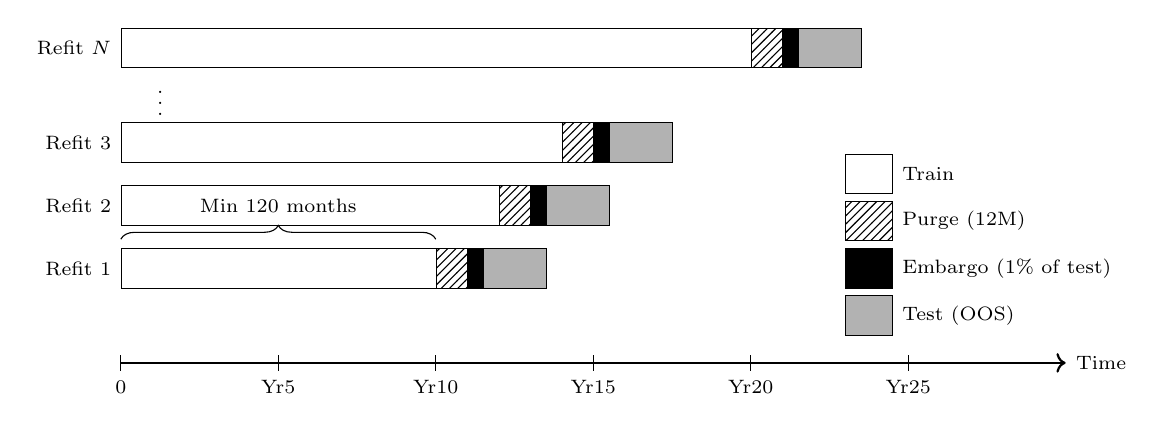
\begin{tikzpicture}[
    trainblock/.style={rectangle, draw=black, fill=white, minimum height=0.5cm, font=\scriptsize},
    purgeblock/.style={rectangle, draw=black, pattern=north east lines, minimum height=0.5cm, font=\scriptsize},
    embargoblock/.style={rectangle, draw=black, fill=black, minimum height=0.5cm, font=\scriptsize},
    testblock/.style={rectangle, draw=black, fill=black!30, minimum height=0.5cm, font=\scriptsize},
]

% Time axis
\draw[->, thick] (0, 0) -- (12, 0) node[right] {\scriptsize Time};

% Year labels
\foreach \x/\label in {0/0, 2/Yr5, 4/Yr10, 6/Yr15, 8/Yr20, 10/Yr25} {
    \draw (\x, -0.1) -- (\x, 0.1);
    \node[below, font=\scriptsize] at (\x, -0.1) {\label};
}

% Refit 1: Year 10
\node[trainblock, minimum width=4cm, anchor=west] at (0, 1.2) {};
\node[purgeblock, minimum width=0.4cm, anchor=west] at (4, 1.2) {};
\node[embargoblock, minimum width=0.2cm, anchor=west] at (4.4, 1.2) {};
\node[testblock, minimum width=0.8cm, anchor=west] at (4.6, 1.2) {};
\node[left, font=\scriptsize] at (0, 1.2) {Refit 1};

% Refit 2: Year 11
\node[trainblock, minimum width=4.8cm, anchor=west] at (0, 2) {};
\node[purgeblock, minimum width=0.4cm, anchor=west] at (4.8, 2) {};
\node[embargoblock, minimum width=0.2cm, anchor=west] at (5.2, 2) {};
\node[testblock, minimum width=0.8cm, anchor=west] at (5.4, 2) {};
\node[left, font=\scriptsize] at (0, 2) {Refit 2};

% Refit 3: Year 12
\node[trainblock, minimum width=5.6cm, anchor=west] at (0, 2.8) {};
\node[purgeblock, minimum width=0.4cm, anchor=west] at (5.6, 2.8) {};
\node[embargoblock, minimum width=0.2cm, anchor=west] at (6.0, 2.8) {};
\node[testblock, minimum width=0.8cm, anchor=west] at (6.2, 2.8) {};
\node[left, font=\scriptsize] at (0, 2.8) {Refit 3};

% Refit N
\node[font=\scriptsize] at (0.5, 3.4) {$\vdots$};
\node[trainblock, minimum width=8cm, anchor=west] at (0, 4) {};
\node[purgeblock, minimum width=0.4cm, anchor=west] at (8, 4) {};
\node[embargoblock, minimum width=0.2cm, anchor=west] at (8.4, 4) {};
\node[testblock, minimum width=0.8cm, anchor=west] at (8.6, 4) {};
\node[left, font=\scriptsize] at (0, 4) {Refit $N$};

% Legend (positioned higher to avoid axis overlap)
\node[trainblock, minimum width=0.6cm] at (9.5, 2.4) {};
\node[right, font=\scriptsize] at (9.8, 2.4) {Train};
\node[purgeblock, minimum width=0.6cm] at (9.5, 1.8) {};
\node[right, font=\scriptsize] at (9.8, 1.8) {Purge (12M)};
\node[embargoblock, minimum width=0.6cm] at (9.5, 1.2) {};
\node[right, font=\scriptsize] at (9.8, 1.2) {Embargo (1\% of test)};
\node[testblock, minimum width=0.6cm] at (9.5, 0.6) {};
\node[right, font=\scriptsize] at (9.8, 0.6) {Test (OOS)};

% Annotations
\draw[decorate, decoration={brace, amplitude=5pt, raise=2pt}] (0, 1.5) -- (4, 1.5) 
    node[midway, above=8pt, font=\scriptsize] {Min 120 months};

\end{tikzpicture}
\caption{Walk-Forward Backtesting with Purged-Embargoed Cross-Validation. The training window expands over time (white), with a 12-month purge gap (hatched) and 1\% of test data embargo (black) separating training from out-of-sample test periods (gray).}
\label{fig:walk-forward}
\end{figure}

\section{HMM Feature Formulas}
\label{app:hmm-features}

This appendix provides the exact formulas for the 3-dimensional HMM observation vector.

\begin{figure}[H]
\centering
\includegraphics[width=0.85\textwidth]{figures/phase2_hmm_regimes.png}
\caption{HMM regime detection using forward-only filtered probabilities. Top: HRP returns with bear regimes shaded in red, showing successful identification of major drawdown periods (2000--2002, 2008--2009, 2020, 2022). Middle: $P(\text{Bull})$ probability time series used for allocation decisions. Bottom: Downside deviation confirms elevated tail risk during bear regimes.}
\label{fig:hmm-regimes}
\end{figure}

\begin{figure}[H]
\centering
\includegraphics[width=0.9\textwidth]{figures/phase3_xgb_analysis(1).png}
\caption{XGBoost model diagnostics. Top-left: ROC curve demonstrates strong discriminative ability (AUC = 0.806). Top-right: P(Bull) distribution shows clear separation between actual bear and bull periods. Bottom-left: Rolling prediction accuracy is stable ($\sim$75--80\%) except during 2000--2005 when the Dot-com bubble collapse created abrupt regime transitions. Bottom-right: Average pairwise correlation dominates feature importance, confirming that correlation breakdown is the primary bear market signal.}
\label{fig:xgb-analysis}
\end{figure}

\begin{table}[H]
\centering
\caption{Regime Prediction Metrics (Out-of-Sample, 1988--2024)}
\label{tab:xgb}
\begin{tabular}{lr}
\toprule
Metric & Value \\
\midrule
Accuracy & 76.5\% \\
ROC-AUC & 0.806 \\
Bear Precision & 53.1\% \\
Bull Precision & 84.6\% \\
Bear Recall & 54.5\% \\
Bull Recall & 83.8\% \\
\bottomrule
\end{tabular}
\end{table}

\begin{table}[H]
\centering
\caption{Confusion Matrix (Out-of-Sample Predictions, 1988--2024)}
\label{tab:confusion}
\begin{tabular}{lcc}
\toprule
& Predicted Bear & Predicted Bull \\
\midrule
Actual Bear (99 months) & 54 (54.5\%) & 45 (45.5\%) \\
Actual Bull (339 months) & 55 (16.2\%) & 284 (83.8\%) \\
\bottomrule
\end{tabular}
\end{table}

\paragraph{Log Returns.}
\begin{equation}
    \text{log\_return}_t = \ln(1 + r_t^{HRP})
\end{equation}

\paragraph{Rolling Downside Deviation.} Computed over a 6-month window, capturing left-tail risk:
\begin{equation}
    \text{DD}_t = \sqrt{\frac{1}{n} \sum_{s=t-5}^{t} \min(r_s, 0)^2}
\end{equation}
Only negative returns contribute to downside deviation.

\paragraph{Michigan Consumer Sentiment Change.} Year-over-year percentage change, lagged one month:
\begin{equation}
    \text{sent\_change}_t = \frac{ICS_{t-1}}{ICS_{t-13}} - 1
\end{equation}

\section{Liquidity Filter Formulas}
\label{app:liquidity}

The universe construction applies a two-stage liquidity filter within each Fama-French 12 industry:
\begin{equation}
    \mathcal{U}_t = \left\{ i : V^{med}_{i,t} \geq Q_{80\%}(V^{med}_{ind(i),t}) \text{ and } P_{i,t} > \$3 \right\}
\end{equation}
where $V^{med}_{i,t}$ is the rolling 12-month median dollar volume and $Q_{80\%}$ denotes the 80th percentile within each industry.

\paragraph{Dollar Volume Calculation.}
Rolling median dollar volume requires a minimum of 6 valid observations:
\begin{equation}
    V^{med}_{i,t} = \text{median}\left(P_{i,s} \times \text{VOL}_{i,s}\right)_{s=t-11}^{t}, \quad \text{requiring } n \geq 6 \text{ valid obs.}
\end{equation}

\section{Transaction Cost Formulas}
\label{app:tx-costs}

The two-stage industry ETF framework requires matching transaction cost accounting.

\paragraph{Stage 1: Within-Industry Rebalancing.}
Each industry ETF is a value-weighted portfolio. When prices change, weights drift from target:
\begin{equation}
    \text{cost}^{Stage1}_t = \sum_{k=1}^{12} \Omega_{k,t} \times \tau_{k,t}^{within} \times C_{bps}, \quad \tau_{k,t}^{within} = \sum_{i \in k} |w_{i,t}^{Target} - w_{i,t}^{Drifted}|
\end{equation}

\paragraph{Stage 2: HRP Rebalancing Across Industries.}
\begin{equation}
    \text{cost}^{Stage2}_t = \sum_{k=1}^{12} |\Omega_{k,t}^{Target} - \Omega_{k,t}^{Drifted}| \times C_{bps}
\end{equation}

\paragraph{Leverage Overlay Cost.}
When changing leverage, both sides are traded:
\begin{equation}
    \text{cost}^{Leverage}_t = 2 \times |L_t - L_{t-1}| \times C_{bps}
\end{equation}

\paragraph{Financing Cost.}
When leveraged ($L_t > 1$):
\begin{equation}
    \text{cost}^{Financing}_t = \max(L_t - 1, 0) \times s
\end{equation}
where $s = 50$ bps financing spread.

\paragraph{Net Returns.}
\begin{equation}
    r_{net,t} = L_t \cdot r_{HRP,t} + (1-L_t) \cdot r_f - \text{cost}^{Stage1}_t - \text{cost}^{Stage2}_t - \text{cost}^{Leverage}_t - \text{cost}^{Financing}_t
\end{equation}

\paragraph{Expanding Z-Score.} Each feature is standardized using \textit{only past data}:
\begin{equation}
    z_t = \frac{x_t - \bar{x}_{1:t-1}}{\sigma_{1:t-1}}
\end{equation}

\begin{figure}[H]
\centering
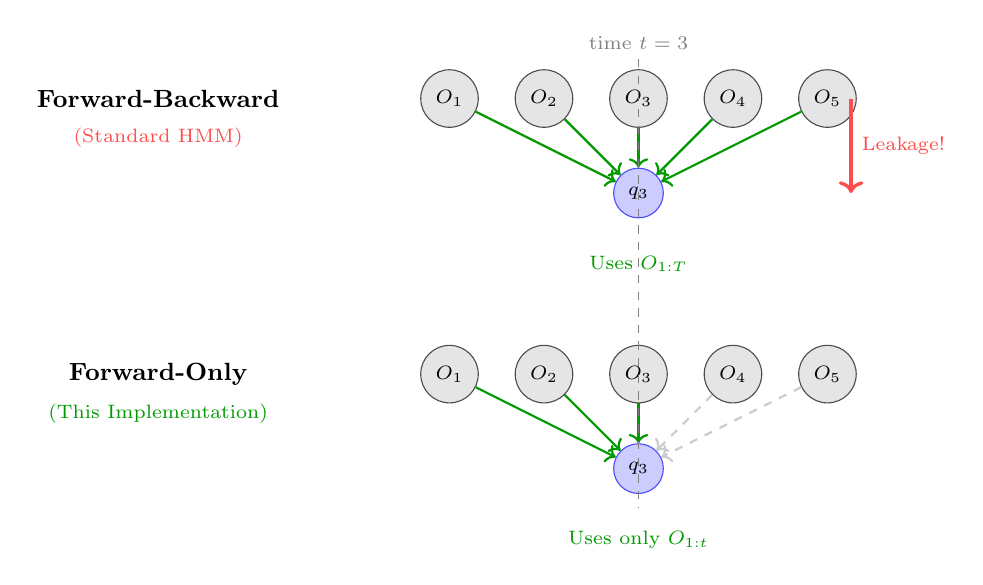
\begin{tikzpicture}[
    obs/.style={circle, draw=black!70, fill=gray!20, minimum size=0.6cm, font=\scriptsize},
    state/.style={circle, draw=blue!70, fill=blue!20, minimum size=0.6cm, font=\scriptsize},
    used/.style={->, thick, green!60!black},
    notused/.style={->, thick, gray!40, dashed},
    leak/.style={->, thick, red!70},
]

% Forward-Backward (top)
\node[font=\small\bfseries] at (-2.5, 2) {Forward-Backward};
\node[font=\scriptsize\color{red!70}] at (-2.5, 1.5) {(Standard HMM)};

% Timeline
\foreach \i in {1,...,5} {
    \node[obs] (fbo\i) at (\i*1.2, 2) {$O_{\i}$};
}
\node[state] (fbq) at (3*1.2, 0.8) {$q_3$};

% Arrows - all observations used
\foreach \i in {1,...,5} {
    \draw[used] (fbo\i) -- (fbq);
}
\node[font=\scriptsize, text=green!60!black] at (3*1.2, -0.1) {Uses $O_{1:T}$};
\draw[leak, very thick] (5*1.2+0.3, 2) -- (5*1.2+0.3, 0.8) node[midway, right, font=\scriptsize, text=red!70] {Leakage!};

% Forward-Only (bottom)
\node[font=\small\bfseries] at (-2.5, -1.5) {Forward-Only};
\node[font=\scriptsize\color{green!60!black}] at (-2.5, -2) {(This Implementation)};

% Timeline
\foreach \i in {1,...,5} {
    \node[obs] (foo\i) at (\i*1.2, -1.5) {$O_{\i}$};
}
\node[state] (foq) at (3*1.2, -2.7) {$q_3$};

% Arrows - only past observations used
\foreach \i in {1,...,3} {
    \draw[used] (foo\i) -- (foq);
}
\foreach \i in {4,...,5} {
    \draw[notused] (foo\i) -- (foq);
}
\node[font=\scriptsize, text=green!60!black] at (3*1.2, -3.6) {Uses only $O_{1:t}$};

% Vertical time indicator
\draw[dashed, gray] (3*1.2, 2.5) -- (3*1.2, -3.2);
\node[font=\scriptsize, gray] at (3*1.2, 2.7) {time $t=3$};

\end{tikzpicture}
\caption{Forward-Backward vs Forward-Only HMM Inference. The standard forward-backward algorithm (top) computes $P(q_t | O_{1:T})$ using all observations including future ones---a severe form of look-ahead bias. The forward-only filter (bottom) computes $P(q_t | O_{1:t})$ using only observations up to time $t$, ensuring no information leakage.}
\label{fig:forward-filter}
\end{figure}

\section{Complete ML Methodology}
\label{app:ml-methodology}

This appendix provides the complete 6-phase methodology for regime-adaptive portfolio enhancement, expanding on the summary in \Cref{sec:methodology}.

\subsection*{Phase 1: HMM Input Construction}

A 3-dimensional observation vector is constructed for the HMM:
\begin{equation}
    \mathbf{O}_t = \begin{bmatrix} \text{log\_return}_t^z \\ \text{downside\_dev}_t^z \\ \text{sent\_change}_t^z \end{bmatrix}
\end{equation}
The three features capture momentum (log returns), left-tail risk (6-month rolling downside deviation), and consumer confidence (YoY sentiment change). See \Cref{app:hmm-features} for exact formulas.

\subsection*{Phase 2: HMM Regime Identification}

Market regimes are modeled as a 2-state Gaussian HMM with parameters $\boldsymbol{\theta} = (\boldsymbol{\pi}, \mathbf{A}, \boldsymbol{\mu}_0, \boldsymbol{\Sigma}_0, \boldsymbol{\mu}_1, \boldsymbol{\Sigma}_1)$, where $\boldsymbol{\mu}_k \in \mathbb{R}^3$ and $\boldsymbol{\Sigma}_k \in \mathbb{R}^{3 \times 3}$.

\paragraph{Forward-Only Filter.} Filtered posteriors are computed as:
\begin{equation}
    P(q_t = j | O_{1:t}) = \frac{\alpha_t(j)}{\sum_{k} \alpha_t(k)}
\end{equation}
where $\alpha_t(j) = P(O_t | q_t = j) \sum_{i} \alpha_{t-1}(i) \cdot A_{ij}$.

\paragraph{Expanding-Window Fitting.} The HMM is re-estimated every 12 months using all available data up to time $t$, starting after 120 months minimum training.

\subsection*{Phase 3: Feature Engineering}

13 predictive features are constructed across four categories:

\begin{table}[H]
\centering
\caption{Feature Categories and Descriptions}
\label{tab:features-app}
\begin{tabular}{lllc}
\toprule
Category & Feature & Description & Z Window \\
\midrule
Cross-sectional & \texttt{dispersion\_z} & Cross-sectional return std & 36M \\
& \texttt{amihud\_z} & Median Amihud illiquidity & 36M \\
& \texttt{bab\_z} & BAB factor 12M momentum & 60M \\
& \texttt{avg\_pairwise\_corr\_z} & Variance ratio proxy & 60M \\
\midrule
Macro & \texttt{credit\_spread} & BAA $-$ 10Y Treasury & 60M \\
& \texttt{term\_spread} & 10Y $-$ 3M Treasury & 60M \\
& \texttt{cpi\_vol} & CPI 24M rolling volatility & 60M \\
& \texttt{m2\_growth} & M2 YoY growth & 60M \\
& \texttt{unrate\_trend} & UNRATE deviation from 12M MA & 60M \\
\midrule
Factor & \texttt{valuation\_spread\_z} & Value spread log(Q5/Q1 B/M) & 60M \\
\midrule
Strategy & \texttt{hrp\_mom\_1m\_z} & 1-month HRP return & 24M \\
Momentum & \texttt{hrp\_mom\_3m\_z} & 3-month cumulative return & 24M \\
& \texttt{hrp\_mom\_12m\_z} & 12-month cumulative return & 24M \\
\bottomrule
\end{tabular}
\end{table}

\paragraph{Target Variable.} Features at time $t$ predict the regime at time $t+1$: $y_t = \text{regime}_{t+1}$.

\subsection*{Phase 4: Walk-Forward XGBoost Prediction}

\paragraph{Hyperparameters.} Following Gu, Kelly, and Xiu \cite{gu2020}: \texttt{max\_depth}=3, \texttt{learning\_rate}=0.05, \texttt{n\_estimators}=500, \texttt{reg\_alpha}=2, \texttt{reg\_lambda}=5.

\paragraph{Purged Time-Series CV.} Following L\'opez de Prado \cite{prado2018}:
\begin{itemize}
    \item \textbf{purge\_gap} = 12 months: removes observations between train and test folds
    \item \textbf{embargo\_pct} = 1\%: additional buffer after test folds
\end{itemize}

\paragraph{Walk-Forward Protocol.}
\begin{enumerate}
    \item Initialize at month 120 (10 years minimum training)
    \item At each refit point (every 12 months):
    \begin{enumerate}
        \item Winsorize features at 1\%/99\% using training bounds only
        \item Train XGBoost on all available training data
    \end{enumerate}
    \item Generate out-of-sample predictions for next 12 months
    \item Advance window and repeat
\end{enumerate}

\subsection*{Phase 5: Portfolio Overlay}

Two-fund separation \cite{tobin1958} mixes HRP with T-Bills based on bull probability:
\begin{equation}
    L_t = P(\text{Bull}_t) \times \frac{1}{\bar{P}(\text{Bull})}
\end{equation}

\paragraph{Financing Costs.} When $L_t > 1$:
\begin{equation}
    r_{portfolio,t} = \begin{cases}
        L_t \cdot r_{HRP,t} + (1-L_t) \cdot r_f & \text{if } L_t \leq 1 \\
        L_t \cdot r_{HRP,t} - (L_t-1) \cdot (r_f + s) & \text{if } L_t > 1
    \end{cases}
\end{equation}
where $s = 50$ bps financing spread.

\subsection*{Phase 6: Transaction Cost Analysis}

Transaction costs (10 bps per trade) are applied at four stages:
\begin{enumerate}
    \item Within-industry stock rebalancing (value-weighted drift)
    \item Across-industry HRP rebalancing
    \item Leverage overlay adjustments ($2 \times |L_t - L_{t-1}|$)
    \item Financing spreads when leveraged ($L > 1$)
\end{enumerate}

\section{Feature Formulas}
\label{app:features}

This appendix provides the exact formulas used to compute each ML feature. All Z-scored features use the rolling ex-ante formula:
\begin{equation}
    z_t = \frac{x_t - \bar{x}_{t-W:t-1}}{\sigma_{t-W:t-1}}
\end{equation}
where $W$ is the rolling window and the \texttt{shift(1)} ensures no look-ahead bias.

\subsection*{Cross-Sectional Features}

\paragraph{Dispersion (\texttt{dispersion\_z}).}
Cross-sectional standard deviation of stock returns:
\begin{equation}
    \text{dispersion}_t = \sqrt{\frac{1}{N_t}\sum_{i=1}^{N_t}(r_{i,t} - \bar{r}_t)^2}
\end{equation}
where $N_t$ is the number of stocks in the universe at time $t$. Z-scored with 36-month window.

\paragraph{Amihud Illiquidity (\texttt{amihud\_z}).}
Median Amihud \cite{amihud2002} illiquidity ratio across all stocks:
\begin{equation}
    \text{amihud}_t = \text{median}_i\left(\frac{|r_{i,t}|}{\text{DollarVol}_{i,t}} \times 10^6\right)
\end{equation}
where $\text{DollarVol}_{i,t} = P_{i,t} \times \text{Vol}_{i,t}$. Log-transformed, then Z-scored with 36-month window.

\paragraph{Betting Against Beta (\texttt{bab\_z}).}
BAB factor momentum following Frazzini and Pedersen \cite{frazzini2014}:
\begin{enumerate}
    \item Compute rolling 36-month beta for each stock: $\beta_i = \text{Cov}(r_i, r_m)/\text{Var}(r_m)$
    \item Clip betas to $[-5, 5]$ and lag by 2 months to avoid look-ahead
    \item Form BAB factor: Long bottom 20\% beta stocks, short top 20\%
    \item Compute 12-month cumulative log return of BAB factor:
    \begin{equation}
        \text{BAB}_{12m,t} = \sum_{s=t-11}^{t} \ln(1 + r^{BAB}_s)
    \end{equation}
\end{enumerate}
Z-scored with 60-month window.

\paragraph{Average Pairwise Correlation (\texttt{avg\_pairwise\_corr\_z}).}
Variance ratio proxy for average correlation:
\begin{equation}
    \text{AvgCorr}_t \approx \frac{\text{Var}(r_m)_t}{\bar{\text{Var}}(r_i)_t}
\end{equation}
where $\text{Var}(r_m)_t$ is 12-month rolling variance of the value-weighted market return, and $\bar{\text{Var}}(r_i)_t$ is the cross-sectional mean of individual stock rolling variances. Z-scored with 60-month window.

\subsection*{Macroeconomic Features}

Note: CPI, M2, and UNRATE are lagged by 1 month to account for publication delay.

\paragraph{Credit Spread (\texttt{credit\_spread}).}
\begin{equation}
    \text{CreditSpread}_t = \text{BAA}_t - \text{DGS10}_t
\end{equation}
Z-scored with 60-month window.

\paragraph{Term Spread (\texttt{term\_spread}).}
\begin{equation}
    \text{TermSpread}_t = \text{DGS10}_t - \text{TB3MS}_t
\end{equation}
Z-scored with 60-month window.

\paragraph{CPI Volatility (\texttt{cpi\_vol}).}
\begin{equation}
    \text{CPIVol}_t = \sigma_{24m}\left(\frac{\text{CPI}_{t-1} - \text{CPI}_{t-13}}{\text{CPI}_{t-13}}\right)
\end{equation}
24-month rolling standard deviation of year-over-year CPI changes (lagged). Z-scored with 60-month window.

\paragraph{M2 Growth (\texttt{m2\_growth}).}
\begin{equation}
    \text{M2Growth}_t = \frac{\text{M2}_{t-1} - \text{M2}_{t-13}}{\text{M2}_{t-13}}
\end{equation}
Year-over-year M2 money supply growth (lagged). Z-scored with 60-month window.

\paragraph{Unemployment Trend (\texttt{unrate\_trend}).}
\begin{equation}
    \text{UnrateTrend}_t = \text{UNRATE}_{t-1} - \bar{\text{UNRATE}}_{t-13:t-2}
\end{equation}
Deviation of unemployment rate from its 12-month moving average (lagged). Z-scored with 60-month window.

\subsection*{Factor Features}

\paragraph{Valuation Spread (\texttt{valuation\_spread\_z}).}
Log ratio of median book-to-market ratios between value and growth quintiles:
\begin{equation}
    \text{ValSpread}_t = \ln\left(\frac{\text{median}(B/M)_{Q5,t}}{\text{median}(B/M)_{Q1,t}}\right)
\end{equation}
where $Q5$ is the top quintile (value) and $Q1$ is the bottom quintile (growth) sorted by book-to-market. Z-scored with 60-month window.

\subsection*{Strategy Momentum Features}

\paragraph{HRP Momentum 1M (\texttt{hrp\_mom\_1m\_z}).}
\begin{equation}
    \text{Mom}_{1m,t} = r^{HRP}_t
\end{equation}
Z-scored with 24-month window.

\paragraph{HRP Momentum 3M (\texttt{hrp\_mom\_3m\_z}).}
\begin{equation}
    \text{Mom}_{3m,t} = \sum_{s=t-2}^{t} \ln(1 + r^{HRP}_s)
\end{equation}
3-month cumulative log return. Z-scored with 24-month window.

\paragraph{HRP Momentum 12M (\texttt{hrp\_mom\_12m\_z}).}
\begin{equation}
    \text{Mom}_{12m,t} = \sum_{s=t-11}^{t} \ln(1 + r^{HRP}_s)
\end{equation}
12-month cumulative log return. Z-scored with 24-month window.

\section{Drawdown Analysis}
\label{app:drawdown-analysis}

\begin{figure}[H]
\centering
\includegraphics[width=0.85\textwidth]{figures/subsample_sharpe_stability.png}
\caption{Sharpe ratio comparison across three subperiods. P(Bull) Scaled consistently outperforms both static HRP and CRSP VW in all subsamples, demonstrating robust performance across different market environments.}
\label{fig:subsample-sharpe}
\end{figure}

\begin{figure}[H]
\centering
\includegraphics[width=0.85\textwidth]{figures/subsample_equity_curves.png}
\caption{Log-scale equity curves across three subperiods. Each panel shows cumulative returns for P(Bull) Scaled, Static HRP, and CRSP VW, illustrating consistent outperformance of the regime-adaptive strategy.}
\label{fig:subsample-equity}
\end{figure}

\begin{figure}[H]
\centering
\includegraphics[width=0.85\textwidth]{figures/drawdown_difference(1).png}
\caption{Drawdown comparison between Static HRP and P(Bull) Scaled strategies. Top panel: Month-by-month drawdown difference---positive values indicate P(Bull) Scaled experienced smaller drawdowns. Bottom panel: Cumulative drawdown protection over time. While 26\% of months show P(Bull) with larger drawdowns, these periods are brief and shallow (max excess DD of $-$3.4\%), whereas protection during crises exceeds +39\% (GFC).}
\label{fig:drawdown-diff}
\end{figure}

%==============================================================================
% ACKNOWLEDGMENTS
%==============================================================================
\section*{Acknowledgments}

The author thanks the course instructors for their guidance on machine learning methodology and the WRDS platform for providing access to CRSP and Compustat data.

%==============================================================================
% REFERENCES
%==============================================================================
\bibliographystyle{siamplain}
\bibliography{references}

\end{document}
